\documentclass{article}
\usepackage[T1]{fontenc}
\usepackage[utf8]{inputenc}

\usepackage{cmbright}
\usepackage[T1]{fontenc}

\usepackage{multicol}

\usepackage{amsmath}
\usepackage{amsfonts}
\usepackage{amssymb}
\usepackage{tikz}
\usepackage{graphicx}
\graphicspath{  {./images/} }
\setlength{\parindent}{0pt}
\usepackage{changepage}
\usepackage{physics}
\usepackage{derivative}
\usepackage{bm}
\usepackage[colorlinks=true, linkcolor=blue, urlcolor=blue, citecolor=blue, anchorcolor=blue]{hyperref}

\addtolength{\oddsidemargin}{-.25in}
\addtolength{\textwidth}{0.5in}

\makeatletter
\newcommand*\bigcdot{\mathpalette\bigcdot@{.5}}
\newcommand*\bigcdot@[2]{\mathbin{\vcenter{\hbox{\scalebox{#2}{$\m@th#1\bullet$}}}}}
\makeatother

\DeclareMathOperator{\di}{d\!}
\newcommand*\Eval[3]{\left.#1\right\rvert_{#2}^{#3}}

\newcommand{\uvec}[1]{\boldsymbol{\hat{\textbf{#1}}}}
\newcommand{\vr}[1]{\textbf{#1}}

\newcommand{\thus}[0]{\; \; \longrightarrow \; \;}

\newcommand{\lag}{\mathcal{L}}
\newcommand{\ham}{\mathcal{H}}

\title{SNR Spread Simulations}
\author{Ryan Liu}
\date{Last updated: May 6, 2021}

\begin{document}

\maketitle

\section{Resources Used}

\begin{enumerate}
    \item \url{https://www.ligo.org/science/Publication-ObservingScenario/index.php} (info on aLIGO sensitivities)
\end{enumerate}

\section{Variables to Consider}

We look at four different factors that may impact the SNR of the GW signal: 
\begin{enumerate}
    \setlength{\itemsep}{0pt}
    \item Distance of observation 
    \item Deviation of the waveform from the actual mass
    \item Sensitivity of LIGO
    \item Variability in random noise
\end{enumerate}
While theoretical calculations are likely possible, due to their complexity we rely on numerical simulations from the functions developed in (2.1) and (2.2). 


\section{Results}


\subsection{Distance of Observation}

Gravitational wave signals dissipate as they travel through spacetime, so it would be expected for the SNR to decrease with increasing distance. As suggested by the initial waveform generation function from PyCBC, this should be a simple inverse proportionality. \\

Additionally, greater distance corresponds to a higher redshift -- as the waveform templates are generated without and redshift effect, higher redshifts will furthermore reduce the SNR. \\

\begin{figure}[!htb]
    \center{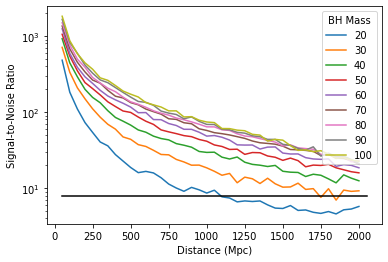
\includegraphics[width=3.5in]{SNR1.png}}
    \caption{\label{fig:massdistance} Maximum SNR of aLIGO at design sensitivity for different black hole masses, assuming the waveform and merger are of the same mass}
\end{figure}

As seen in Figure \ref{fig:massdistance}, at design sensitivity most black hole mergers have a SNR significantly above that expected of random noise from aLIGO up to 2000 Mpc. However, noticeable variations in the expected smooth trend can be seen in the lower masses at large distances.  

\subsection{Imprecise Waveform Masses}

\begin{figure}[!htb]
    \center{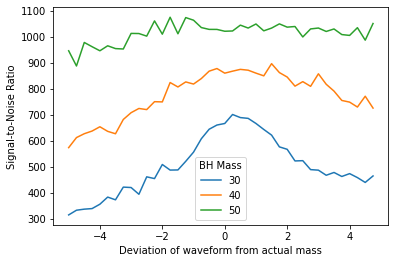
\includegraphics[width=2.8in]{SNR2.png}
    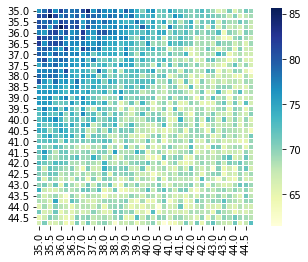
\includegraphics[width=2.2in]{SNR6.png}}
    \caption{\label{fig:waveformspread} (Left) Maximum SNR of aLIGO at design sensitivity and a distance of 500 Mpc with variable template waveforms; (Right) Maximum SNR of a 40 $M_\odot$ BH merger at distance 500 Mpc using different waveform masses}
\end{figure}

Given that the parameters of black hole mergers are not likely to exactly match that of the template waveforms used to detect them, it is important to determine the impact of detecting mergers using imprecise waveforms. From Figure \ref{fig:waveformspread}(a) we can see that the effect is much more pronounced for mergers of smaller black holes. We also notice from Figure \ref{fig:waveformspread}(b) that when varying the waveform template, the highest SNR are achieved when using slightly smaller masses for the template. This is because smaller masses coalesce at a lower frequency, approximating the redshift effect. 

\subsection{LIGO Sensitivity}

\begin{figure}[!htb]
    \center{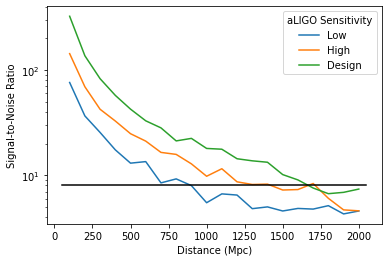
\includegraphics[width=3.5in]{SNR3.png}}
    \caption{\label{fig:sensitivity} Maximum SNR of a $30 M_\odot$ black hole merger at various distances and sensitivities}
\end{figure}

As aLIGO undergoes multiple observing runs, its sensitivity will slowly approach design sensitivity. This is expected to be achieved by 2021. Low and high sensitivities denote estimates for the O1 and O3 runs respectively. \\

As seen in Figure \ref{fig:sensitivity}, as expected SNR increases with improved sensitivity. In the detection frequency range (30 to 1000 Hz), the strain noise is approximately one order of magnitude lower at design sensitivity compared to estimates for the O1 run -- this translated into SNR readings approximately 2 - 3 times higher. 


\subsection{Variability in Random Noise}

\begin{figure}[!htb]
    \begin{center}
        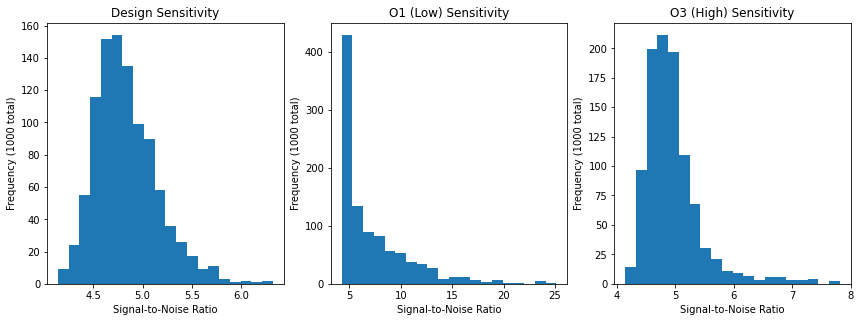
\includegraphics[width=\textwidth]{SNR4.png}
        
        \vspace{5mm}
        
        \begin{tabular}{| c | c | c | c | c | }
            \hline
            Sensitivity & Mean SNR & Std Dev of SNR & Skewness \\
            \hline
            aLIGO Design & 4.83562 & 0.32001 & 0.89421 \\
            O1 (EarlyLow) & 7.26471 & 3.44409 & 1.88561 \\
            03 (EarlyHigh) & 4.95050 & 0.49410 & 2.18882 \\
            \hline
        \end{tabular}
    \end{center}
    
    \caption{\label{fig:noise} Distribution of SNR on 32-second intervals of aLIGO sensitivity Gaussian noise using a $30 M_\odot$ template waveforms}
\end{figure}

By the nature of background noise, different time intervals of both real noise and generated noise will lead to different maximum SNRs, both with and without an actual GW signal. Interestingly, the average value and spread of maximum SNRs given a random waveform template varies significantly at different sensitivities, as seen in Figure \ref{fig:noise}; in particular, the average SNR of the O! run is significantly higher than O3 or aLIGO, which are approximately the same. Additionally, all three distributions have significant rightwards skew, in line with expectations. \\

Similarly, some variation is expected to arise when detecting the same waveform inserted over different randomly generated noise, as seen in Figure \ref{fig:dist}. However, the SNR distribution is only very slightly skewed to the right, likely a product of the large signal size in comparison to the noise.

\begin{figure}
    \begin{center}
        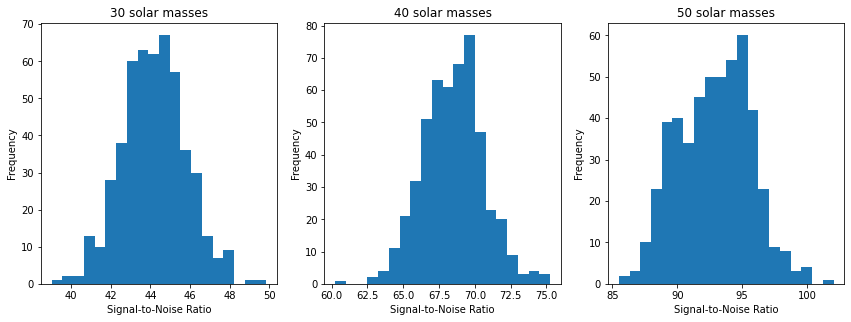
\includegraphics[width=\textwidth]{SNR5.png}
        
        \vspace{5mm}
        
        \begin{tabular}{| c | c | c | c | c | }
            \hline
            BH Mass & Mean SNR & Std Dev of SNR & Skewness \\
            \hline
            30 $M_\odot$ & 44.17599 & 1.60842 & 0.07557 \\
            40 $M_\odot$ & 68.48877 & 2.11456 & 0.00483 \\
            50 $M_\odot$ & 92.87205 & 2.80538 & 0.01637 \\
            \hline
        \end{tabular}
    \end{center}
    
    \caption{\label{fig:dist} Distribution of the SNR produced by a black hole merger with the same template waveform at aLIGO design sensitivity}
\end{figure}



\end{document}